\documentclass[12pt,twoside]{report}


%%%%%%%%%%%%%%%%%%%%%%%%%%%%%%%%%%%%%%%%%%%%%%%%%%%%%%%%%%%%%%%%%%%%%%%%%%%%%

% Definitions for the title page
% Edit these to provide the correct information
% e.g. \newcommand{\reportauthor}{Timothy Kimber}

\newcommand{\reporttitle}{ Gaussian Processes for \\ Optimal Sensor Position \\[0.5cm] { \Large  Background \& Progress Report}}
\newcommand{\reportauthor}{Adrian \textsc{Löwenstein} \\ \phantom{blank author} }
\newcommand{\supervisor}{Rossella \textsc{Arcucci} \\ Miguel \textsc{Molina-Solana}}

\newcommand{\degreetype}{Computing (Machine Learning)}

%%%%%%%%%%%%%%%%%%%%%%%%%%%%%%%%%%%%%%%%%%%%%%%%%%%%%%%%%%%%%%%%%%%%%%%%%%%%%

% load some definitions and default packages
%%%%%%%%%%%%%%%%%%%%%%%%%%%%%%%%%%%%%%%%%
% University Assignment Title Page 
% LaTeX Template
% Version 1.0 (27/12/12)
%
% This template has been downloaded from:
% http://www.LaTeXTemplates.com
%
% Original author:
% WikiBooks (http://en.wikibooks.org/wiki/LaTeX/Title_Creation)
%
% License:
% CC BY-NC-SA 3.0 (http://creativecommons.org/licenses/by-nc-sa/3.0/)
% 
%
%%%%%%%%%%%%%%%%%%%%%%%%%%%%%%%%%%%%%%%%%
%----------------------------------------------------------------------------------------
%	PACKAGES AND OTHER DOCUMENT CONFIGURATIONS
%----------------------------------------------------------------------------------------
\usepackage[a4paper,hmargin=2.8cm,vmargin=2.0cm,includeheadfoot]{geometry}
\usepackage{caption}
\usepackage{subcaption}
\usepackage{textpos}
\usepackage{natbib} % for bibliography
\usepackage{tabularx,longtable,multirow}%hangcaption
\usepackage{fncylab} %formatting of labels
\usepackage{fancyhdr} % page layout
\usepackage{url} % URLs
\usepackage[english]{babel}
\usepackage{amsmath}
\usepackage{graphicx}
\usepackage{dsfont}
\usepackage{epstopdf} % automatically replace .eps with .pdf in graphics
\usepackage{backref} % needed for citations
\usepackage{array}
\usepackage{latexsym}
\usepackage[pdftex,pagebackref,hypertexnames=false,colorlinks]{hyperref} 
% provide links in pdf



\hypersetup{pdftitle={},
  pdfsubject={}, 
  pdfauthor={},
  pdfkeywords={}, 
  pdfstartview=FitH,
  pdfpagemode={UseOutlines},% None, FullScreen, UseOutlines
  bookmarksnumbered=true, bookmarksopen=true, colorlinks,
    citecolor=black,%
    filecolor=black,%
    linkcolor=black,%
    urlcolor=black}

\usepackage[all]{hypcap}


%\usepackage{color}
%\usepackage[tight,ugly]{units}
%\usepackage{float}
%\usepackage{tcolorbox}
%\usepackage[colorinlistoftodos]{todonotes}
% \usepackage{ntheorem}
% \theoremstyle{break}
% \newtheorem{lemma}{Lemma}
% \newtheorem{theorem}{Theorem}
% \newtheorem{remark}{Remark}
% \newtheorem{definition}{Definition}
% \newtheorem{proof}{Proof}


%%% Default fonts
\renewcommand*{\rmdefault}{bch}
\renewcommand*{\ttdefault}{cmtt}



%%% Default settings (page layout)
\setlength{\parindent}{0em}  % indentation of paragraph

\setlength{\headheight}{14.5pt}
\pagestyle{fancy}
\renewcommand{\chaptermark}[1]{\markboth{\chaptername\ \thechapter.\ #1}{}} 

\fancyfoot[ER,OL]{\sffamily\textbf{\thepage}}%Page no. in the left on odd pages and on right on even pages
\fancyfoot[OC,EC]{\sffamily }
\renewcommand{\headrulewidth}{0.1pt}
\renewcommand{\footrulewidth}{0.1pt}
\captionsetup{margin=10pt,font=small,labelfont=bf}


%--- chapter heading

\def\@makechapterhead#1{%
  \vspace*{10\p@}%
  {\parindent \z@ \raggedright \sffamily
    \interlinepenalty\@M
    \Huge\bfseries \thechapter \space\space #1\par\nobreak
    \vskip 30\p@
  }}

%---chapter heading for \chapter*  
\def\@makeschapterhead#1{%
  \vspace*{10\p@}%
  {\parindent \z@ \raggedright
    \sffamily
    \interlinepenalty\@M
    \Huge \bfseries  #1\par\nobreak
    \vskip 30\p@
  }}

\allowdisplaybreaks

% load some macros
% Here, you can define your own macros. Some examples are given below.

\newcommand{\R}[0]{\mathds{R}} % real numbers
\newcommand{\Z}[0]{\mathds{Z}} % integers
\newcommand{\N}[0]{\mathds{N}} % natural numbers
\newcommand{\C}[0]{\mathds{C}} % complex numbers
\renewcommand{\vec}[1]{{\boldsymbol{{#1}}}} % vector
\newcommand{\mat}[1]{{\boldsymbol{{#1}}}} % matrix
\newcommand{\norm}[1]{\left\lVert#1\right\rVert}


\date{June 2019}

\begin{document}

% load title page
% Last modification: 2015-08-17 (Marc Deisenroth)
\begin{titlepage}

\newcommand{\HRule}{\rule{\linewidth}{0.5mm}} % Defines a new command for the horizontal lines, change thickness here


%----------------------------------------------------------------------------------------
%	LOGO SECTION
%----------------------------------------------------------------------------------------


\includegraphics[width = 4cm]{./figures/imperial}\\[0.5cm] 

\center % Center remainder of the page

%----------------------------------------------------------------------------------------
%	HEADING SECTIONS
%----------------------------------------------------------------------------------------

\textsc{\Large Imperial College London}\\[0.5cm] 
\textsc{\large Department of Computing}\\[0.5cm] 

%----------------------------------------------------------------------------------------
%	TITLE SECTION
%----------------------------------------------------------------------------------------

\HRule \\[0.4cm]
{ \huge \bfseries \reporttitle}\\ % Title of your document
\HRule \\[1.5cm]
 
%----------------------------------------------------------------------------------------
%	AUTHOR SECTION
%----------------------------------------------------------------------------------------

\begin{minipage}{0.4\textwidth}
\begin{flushleft} \large
\emph{Author:}\\
\reportauthor % Your name
\end{flushleft}
\end{minipage}
~
\begin{minipage}{0.4\textwidth}
\begin{flushright} \large
\emph{Supervisor:} \\
\supervisor % Supervisor's Name
\end{flushright}
\end{minipage}\\[4cm]


%----------------------------------------------------------------------------------------
%	FOOTER & DATE SECTION
%----------------------------------------------------------------------------------------
\vfill % Fill the rest of the page with whitespace
Submitted in partial fulfillment of the requirements for the MSc degree in
\degreetype~of Imperial College London\\[0.5cm]

\makeatletter
\@date 
\makeatother


\end{titlepage}



% page numbering etc.
\pagenumbering{roman}
\clearpage{\pagestyle{empty}\cleardoublepage}
\setcounter{page}{1}
\pagestyle{fancy}

%%%%%%%%%%%%%%%%%%%%%%%%%%%%%%%%%%%%
%\begin{abstract}
%Your abstract.
%\end{abstract}

\cleardoublepage
%%%%%%%%%%%%%%%%%%%%%%%%%%%%%%%%%%%%
%\section*{Acknowledgments}
%Comment this out if not needed.

\clearpage{\pagestyle{empty}\cleardoublepage}

%%%%%%%%%%% TABLE OF CONTENTS 

%--- table of contents
\fancyhead[RE,LO]{\sffamily {Table of Contents}}
\tableofcontents 


\clearpage{\pagestyle{empty}\cleardoublepage}
\pagenumbering{arabic}
\setcounter{page}{1}
\fancyhead[LE,RO]{\slshape \rightmark}
\fancyhead[LO,RE]{\slshape \leftmark}

\pagebreak
%%%%%%%%%%% TABLE OF TODO's

\listoftodos



%%%%%%%%%%% CHAPTER : INTRODUCTION
\chapter{Introduction}

\todo{Write a proper Introduction}


\paragraph{Project Proposal:}
Gaussian processes (GP) have been widely used since the 1970s in the fields of geostatistics and meteorology. Current applications are in diverse fields including sensor placement
In this project, we propose the employment of a GP model to calculate the optimal spatial positioning of sensors to study and collect air pollution data in big cities. We will then validate the results by means of a data assimilation software with the data at the proposed positions.

\paragraph{Dataset:} London South Bank University (LSBU) air pollution data (velocity, tracer)



 
%%%%%%%%%%% CHAPTER : BACKGROUND
\chapter{Background}

In this chapter, we will cover the literature and the theory that will be used throughout the project. First, we will review the context of the project and how it fits into the \textbf{MAGIC} project. Then our focus goes to the definition of \textbf{Gaussian Processes} (GP) and how they are used in the context of geospatial data. Furthermore, the use of GP relies heavily on \textbf{Covariance} matrixes which need to be estimated. Those tools enable us to create \textbf{optimisation} algorithms for the position of sensors. Finally, we will quickly explore the concepts of \textbf{Data Assimilation} (DA) that will be used to validate the results of the optimisation. 

\section{The MAGIC Project}

This work is done in the context of the \textbf{Managing Air for Green Inner Cities} project. This is a multidisciplinary project and has for objective to find solutions to the pollution and heating phenomenons in cities. Traditionally, urban environmental control relies on polluting and energy consuming heating, ventilation and cooling (HVAC) systems. The usage of the systems increases the heat and the pollution levels, inducing an increased need for the HVAC. The MAGIC project aims at breaking this vicious circle and has for objective to provide tools to make possible the design of cities acting as a natural HVAC system. \\


This has been extensively discussed by  \cite{song_natural_2018}.  For this purpose, integrated management and the decision-support system is under development. It includes a variety of simulations for pollutants and temperature at different scales; a set of mathematical tools to allow fast computation in the context of real-time analysis; and cost-benefit models to asses the viability of the planning options and decisions. \\

As explained by \cite{song_natural_2018}, the test site which has been selected to conduct the study is a real urban area located in London South Bank University (LSBU) in  Elephant and Castle, London. In order to investigate the effect of ventilation on the cities problem, researchers in the MAGIC project have created simulations and experiments both in outdoor and indoor conditions, on the test site. They used wind tunnel experiments and computational fluid dynamics (CFD) to simulate the outdoor environment. Further works include the development of reduced-order modelling (ROM) in order to make faster the simulations while keeping a high level of accuracy \citep{arcucci_effective_2018}. \\

Another key research direction in the use Data Assimilation (DA) and more specifically Variational DA (VarDA) for assimilating measured data in real time and allowing better prediction of the model in the near future \citep{arcucci_effective_2018}. The further use of those methods would be the optimisation of the position of the sensors which provide information for the VarDA.


\section{Gaussian Processes}

In this chapter, we will review Gaussian Processes (GP) which are probabilistic models for spatial predictions based on observations assumption. \\ 

As explained by \citet[p.~29]{rasmussen_gaussian_2006}, the history of Gaussian Processes goes back at least as far as the 1940s. A lot of usages were developed in various fields. Notably for predictions in spatial statistics \citep{cressie_statistics_1991}.  Applied in particular in Geostatistics with methods known as \textit{kringing}, and in Meteorology. Gradually GP started to be used in more general cases for regression. Nowadays it is often used in the context of Machine Learning. \\


For our problem, we will be modelling the data of the sensor with GPs.
%As for sensor optimisation, we will follow the approach that was developed by \citet{krause_near-optimal_2008}. This method relies on GP for finding a near-optimal solution to the problem of placing sensors. 

\todo{Mention the main assumption that the data needs to be gaussianly distributed and iid samples (Maybe already explained)}

\subsection{Sensor Data Modelling}

\subsubsection{Multivariate Gaussian Distribution}

GP will serve as a basic tool in our project. In the space we are monitoring we have a certain number of sensors measuring a certain quantity, such as temperature, pressure, speed of the wind or the concentration of a pollutant at a given position. We assume that the measured quantity has a \textit{multivariate Gaussian joint distribution} between each point of the space. The associated random variable is $\X_\V$ for the set of locations $\V$ we would have the following distribution : $P(\X_\V = \vec{x}_\V) \sim \mathcal{N}(\mu_\V, K_{\V\V}) $, or explicitly : 


\begin{equation}
    P(\X_\V = \vec{x}_\V) \frac{1}{(2\pi)^{n/2} |K_{\V\V}|} \exp^{-\frac{1}{2}(\vec{x}_\V - \mu_\V)^T K_{\V\V}^{-1} (\vec{x}_\V - \mu_\V)}
\end{equation}


\subsubsection{Prediction with Gaussian Processes}
Let us still consider that we have the set of locations $\V$ and a set of sensors $\A$. In order to predict the quantity at positions were we have no sensors ($\V \backslash \A $) we can use a Gaussian Process. This allows us to infer a function belonging the the function space : $\mathcal{GP}(\mathcal{M}(\vec{x}), \mathcal{K}(\vec{x},\vec{x}'))$.  This GP is associated with a \textbf{mean function} $\mathcal{M}(\cdot)$ and a symmetric positive-definite \textbf{kernel function} $\mathcal{K}(\cdot,\cdot)$. We will denote the mean function values for a set of positions $\A$ by $\mu_\A$ and the kernel function values, or covariance matrix, between those points by $K_\A$. More detailed definitions are available in \citet[p.~13-16]{rasmussen_gaussian_2006}. \\

For a set of observations $\vec{x}_\A$ at positions $\A$ we can express for a finite set of other positions $\V \backslash \A $ the conditional distribution of those values. This means that we are able, for each point $y \in \V \backslash \A $, to predict the mean and the variance of $\vec{x}_y$. Using conditional distribution for the Multivariate Gaussian Distribution \citep[p.~193]{deisenroth_mathematics_2018}, we are able to express the following : 
\begin{align}
    P(\X_y | \vec{x}_\A ) &= \mathcal{N}(\mu_{y | \A}, K_{y | \A}) \\
    \mu_{y | \A} &= \mu_y + K_{y\A} K_{\A\A}^{-1} (y - \mu_y)\\ 
    K_{y | \A} &=  K_{yy} - K_{y\A} K_{\A\A}^{-1} K_{\A y} \label{equ:covGP}
\end{align}

An important point to notice is that the predicted covariance for the point y is not dependent of the values measured at $\A$, this is really useful because it allows us to define the uncertainty at $y$ without using only the covariance. \\

\subsection{Scalable Gaussian Processes} 

The biggest weakness of Standard GPs is their complexity. For $p$ training points, the algorithm requires the inversion of a $p \times p$ covariance matrix $K_{pp}$. \citet{liu_when_2018} gives an extensive review of all methods used to make the GPs more scalable. Those methods are evaluated with regards to their \textit{scalability} and their \textit{capability}. \\ 

We redefine notations used here to expose scalable Gaussian Processes.  We consider $n$ training points $\mathbf{X}= \{\vec{x}_i \in \mathbb{R}^d \}^n_{i=1}$, and observations $\vec{y} = \{y_i = y(\vec{x}_i) \in \mathbb{R} \}^n_{i=1} $. GP aims at inferring the function $f : \mathbb{R}^d \mapsto \mathbb{R}$ that describes the best the training data. This function belongs to the  function space $\mathcal{GP}(\mathcal{M}(\vec{x}), \mathcal{K}(\vec{x},\vec{x}'))$. We then replace the conditionals .  In order to obtain the observations we formally add gaussian noise $\mathcal{N}(0,\epsilon_nI_n)$ to the inferred function values (we didn't need that in the previous section). 
\subsubsection{Global Approaches}

The aim of global approximation is to reduce the size of the covariance matrix, in order to make the computation scalable. There are several ways to proceed: \textbf{subset of data} method where we reduce the size of the training set; the \textbf{sparse kernel} methods where we exploit a low-rank representation of the GP (\textbf{sparse approximation}). \\ 


The \textbf{subset of data method} (SoD) is a very simple strategy that only requires to create a subset of the original training data. The resulting cost of the GP is only of $\mathcal{O}(m^3)$ with $m$ the number of points in the subset and $m << p$.  \\

The \textbf{sparse kernel} approach is the idea to reduce the importance of the points far from each other and imposing sparsity of the covariance by setting to zero the elements of the matrix $K_{pp}$ that are below a certain threshold. The resulting complexity being of $\mathcal{O}(\alpha p^3)$ with $0 < \alpha < 1$. The difficulty here is to ensure the positive definiteness of the resulting covariance. Methods for obtaining such results are discussed in the next section. \\

The \textbf{sparse approximation} methods are very diverse and are allowed by different kinds of approximations : the \textbf{approximation of the prior} ; the \textbf{approximation of the posterior} ; \textbf{structured sparse approximations}. \\

\textbf{Prior approximation} modifies the joint prior $p(\mathit{f,f_*})$ between the training data $\mathit{f}_*$ and the test data $\mathit{f}$ by assuming independence between them knowing \textbf{inducing variables} $\mathit{f}_m$ : $\mathit{f}_* \perp \mathit{f} \; | \; \mathit{f}_m$. We also define the Nyström notation for the covariance : $\vec{Q}_{ab} = \vec{K}_{am} \vec{K}_{mm}^{-1} \vec{K}_{mb} $. We are then able to express the conditional probabilities for $p(\mathit{f} | \mathit{f}_m) = \mathcal{N}(\mathit{f} \; | \; \vec{K}_{nm}\vec{K}_{mm}^{-1}\mathit{f}_m \, , \vec{K}_{nn} - \vec{Q}_{nn})$ and  $p(\mathit{f}_* | \mathit{f}_m)  = \mathcal{N}(\mathit{f} \; | \; \vec{K}_{*m}\vec{K}_{mm}^{-1}\mathit{f}_* \, , \vec{K}_{**} - \vec{Q}_{**})$  and approximate them to : $q(\mathit{f} | \mathit{f}_m)$ and  $q(\mathit{f}_* | \mathit{f}_m)$ by replacing respectively the covariances by   $\tilde{\vec{Q}}_{nn}$ and $\tilde{\vec{Q}}_{**}$. This approximation allows for a computation with a reduced complexity of $\mathcal{O}(mn^2)$. \\

 In order to select an appropriate approximate covariance $\tilde{\vec{Q}}_{nn}$ and $\tilde{\vec{Q}}_{**}$, different methods are referenced such as  SoR, DTC, FITC and PITC. 
 
 \textit{Subset of Regressor} (SoR) fixes both covariances to $0$, forcing a deterministic view. 
 
 In the \textit{Deterministic Training Conditional} (DTC), imposes a deterministic training $\tilde{\vec{Q}}_{nn} = 0$ but keeps the exact test conditional $p(\mathit{f}_* | \mathit{f}_m)$. 
 
 Another approach is the \textit{Fully Independent Training Conditional} (FITC). Here we keep exact the test conditional but we approximate the training by considering that each realisation is independent from each other : the $\{\mathit{f}_i\}^n_{i=1}$ are fully independent, and we take the covariance to be $\tilde{\vec{Q}}_{nn} = diag(\vec{K}_{nn} - \vec{Q}_{nn} ) $. This leads to better results than the two previous methods. 
 In order to further improve this method the idea of \textit{Partially Independent Training Conditional} (PITC) was introduced. Here we consider that not all the training points are independent, but only some of them. This leads to an independence by blocks, and an block-diagonal covariance approximation : $\tilde{\vec{Q}}_{nn} = blkdiag(\vec{K}_{nn} - \vec{Q}_{nn} ) $. 
 
In those methods, the choice of the $m$ \textit{inducing points} is crucial to enable a good approximation. \\


Another way to see the problem is to \textbf{approximate the posterior} $p(\mathit{f,f_*} | \vec{y})$ of the GP instead of the prior $p(\mathit{f,f_*})$, by replacing it with a variational distribution  $q(\mathit{f,f_*} | \vec{y})$. The main method is called the \textit{Variational Free Energy} (VFE), and has been developed by \cite{titsias_variational_2009}. We optimise the variational parameters and hyperparameters of the  approximation by minimising the KL divergence between the two distributions : 


\begin{align}
    KL(q(\mathit{f,f_*} | \vec{y})\; || \;  p(\mathit{f,f_*} | \vec{y})) &= \log p(\vec{y}) - \left\langle  \log \frac{p(\mathit{f,f_*},\vec{y})}{q(\mathit{f,f_*} | \vec{y})}\right\rangle_{q(\mathit{f,f_*} | \vec{y})} \\
    &= \log p(\vec{y}) - F_q
    \label{equ:vfe_kl}
    \end{align}  
    
As the KL divergence is positive, minimising this quantity is equivalent to maximising the Variational Free Energy (VFE): $F_q$ (also called Evidence Lower Bound - ELBO). A tighter bound can be derived to replace $F_q$ : 
\begin{equation}
    F_{VFE} = \log q_{DTC}(\vec{y}) - \frac{1}{2\sigma_\epsilon^2} tr(\vec{K}_{nn} - \vec{Q}_{nn})
\end{equation}

In the DTC we maximised the likelihood $q_{DTC}(\vec{y})$ and here we add only an additional term. This has 3 functions: it acts as a regulariser against over-fitting; it helps finding a good inducing set; it always improves the ELBO with increasing $m$.  \\

Finally, the last global approach is the \textit{structured sparse approximations}. The main idea is to speed up the computation of the inversion of the covariance matrix and multiplication by a vector: $\vec{K}_{nn}^{-1}\vec{y}$. For that fast \textit{matrix vector multiplication} (MVM) is used, it solves the linear system by using conjugate gradients. Several improvements have been proposed, especially when the covariance matrix $\vec{K}_{nn}$ has some algebraic structure, such as in the \textit{Kroenecker Methods} and the \textit{Toeplitz Methods}. Those methods require also inputs having a grid structure, therefore not directly applicable in our project.  In order to generalise those methods to any kind of data structure, the method of structured kernel interpolation (SKI) was also proposed by \citet{wilson_kernel_2015}. Inducing points are created using local linear interpolation techniques and constrained to the grid structure. This method has drawbacks such as exponential growth of inducing points in high dimension; discontinuous predictions and overconfident variance. 


\subsubsection{Local Approaches}

Applying the principle de Divide and Conquer (D\&C), the main idea is to use \textit{local experts} to create a full GP representation. It has the main advantage to enable naturally \textit{parallelisation} and to capture \textit{non-stationary} features. We can use naive local experts (NLE), or more complex combinations of localised experts such as mixture of experts (MoE) or Products of Experts (PoE). \\

In naive local experts (NLE), each expert is trained on a different subset of the space. For a training set of points $\mathcal{D}$ and its subsets $\mathcal{D}_i$, we have the prediction of the expert $\mathcal{M}_i$ inside a subregion $\Omega_i$ : $\vec{x}_* \in \Omega_i$ such as $p(y_* | \mathcal{D}, \vec{x}_*) \approx p_i(y_* | \mathcal{D}_i, \vec{x}_*) $. In \textit{inductive} NLE, the space is first partitioned and each expert is trained before choosing the appropriate one of the prediction. The partition is therefore fixed beforehand. In \textit{transductive} NLE, once the prediction point $\vec{x}_*$ has been chosen,  the expert $\mathcal{M}_*$ is trained locally on a subset $\mathcal{D}_*$ close to $\vec{x}_*$. A few drawbacks are the discontinuities at the boundaries between the subregions and the fact that it generalises badly to all the regions. \\

\textbf{Note :} This section will be developed further as the project explores those methods in practice especially MoE and PoE. 

\subsection{Covariance Matrix Estimation} \label{sec:cov_est}

We have seen how GPs are defined and made more scalable. In order to have good results, we need to have a good estimate of the covariance matrix between the points of our space. \\



%Many application requires the covariance to be estimated because of the lack of measures. Very often a limited number of sensors has been in position and the key challenge is to interpolate the covariance. talk of the different methods\\

In our specific case, we already have at our disposal a very dense network of measurement. With more than $100'000$ different locations we don't need to explore the space outside of those points. Unfortunately, the sample covariance is a very bad estimator of the true covariance in high dimensional settings such as ours \citep{pourahmadi_covariance_2011}. \\


We will see the properties that our covariance to accurately model our space, before discussing the best ways of estimating the covariance matrix estimation.


\subsubsection{Properties of Covariance}

By definition a covariance matrix must be \textbf{positive-definite} and \textbf{symmetrical} \citep[p.~80]{rasmussen_gaussian_2006}. \\

A covariance function between two inputs $x$ and $x'$ is \textbf{stationary}   when it is invariant to translation. Thus, when it is a function of $x' - x$. \\
In a covariance function that is \textbf{isotropic}, we remove the dependence of the direction and, it becomes a function of the distance between the two points: $|x' - x|$. The isotropy of the covariance function is a stronger assumption than  \\ 

In our problem, we can't assume that the process is stationary nor isotropic. Our space is 3-dimensional and not homogeneous. The presence of the buildings and other obstacles that likely to make environment variables less smooth \citep{paciorek_nonstationary_2004}. Also, it has been shown by \citet{krause_near-optimal_2008} that non-stationary covariance matrixes give better results than stationary or isotropic. This makes us choose a non-stationary covariance matrix for the  GPs of our problem.


\subsubsection{Covariance Estimation}

We consider the process $Y$ in $p$ different locations at $T$ sampling times. $\vec{Y}_t = (Y_{1t}, \dots, Y_{pt})$, with $t = 1 \dots T$. We want to estimate the covariance matrix $\Sigma$. \\

\paragraph{Sample Covariance}

The simplest estimator of the covariance matrix is the \textbf{sample covariance matrix} $\vec{S}$ directly computed from the captured data. 

\begin{equation}
    \vec{S} = \frac{1}{T -1} \sum_{t=1}^T (\vec{Y}_t - \bar{\vec{Y}})\cdot (\vec{Y}_t - \bar{\vec{Y}}_t)^T, \quad \bar{\vec{Y}} = \frac{1}{T} \sum_{t=1}^T \vec{Y}_t
\end{equation}

Unfortunately, this covariance is singular when $p >> T$ \citep{fan_overview_2015}, and the accumulation of errors due to the number of parameters to estimate. One additional assumption that we need to make for this covariance is its the sparsity of the covariance which is needed to reduce the number of parameters and is often realistic in practice. 

\paragraph{Shrinkage Methods}
%
%\paragraph{Estimating a Spatial Covariance} 
%
%\cite{nott_estimation_2002-1} proposed to fit local variograms in order to approaximate the covariance matrix. It is a method that was developped in \cite{cressie_statistics_1991}. \\
%
%Another method is the use of spatial deformation of the kernel in order to obtain non-stationarity \citep{sampson_nonparametric_1992}. \\
%
%Several different approaches are developed in the literature, notably the works of \citep{fan_overview_2015} and \cite{guttorp_20_1994} which is more focused on spatial data. 
%
%\textbf{Note :} This section needs further developments, in order to find an implement the best possible approach in \textit{coordination} with the scalable Gaussian Processes. 
%
\todo{Remove this part on spatial covariance, maybe mention it}
\todo{Explain the problem with the nature of the covariance and explain shrinkage methods}


\section{Sensor Position Optimisation}

Now that we have modelled the relationship between the positions using GPS we can establish an algorithm that was developed by \citet{krause_near-optimal_2008}. The process of placing sensors in an optimal way is called in spatial statistics, \textit{sampling} or \textit{experimental design}. We want to find the optimal way to place a number of $k$ sensors (indexed by $\A$) inside the set of possible sensor locations $\S$ . So that we have $\A \subseteq \S \subseteq \V$. \\


For the rest of this section, we assume that we have at our disposal a good estimate of the covariance matrix between each point. In practice this is not that obvious as we have seen in section \ref{sec:cov_est}. The following is valid for any covariance matrix that is symmetric and positive-definite. \\ 

First, we will define how to characterise a good design in term of sensor placement. Then we will define the main optimisation algorithm and its improvements. \\ 

\subsection{Placement Criterion}

\subsubsection{Entropy Criterion}

Intuitively a good way of measuring uncertainty is the \textit{entropy}. By observing the conditional entropy of the location where no sensor was placed $\VA$, we can estimate the uncertainty remaining for those locations. We define the following conditional entropy of the un-instrumented location knowing the instrumented ones \citep[p.~16]{cover_elements_1991} :

\begin{align}
    H(\X_{\VA} | \X_\A) &= \mathbb{E}_{p(\vec{x}_{\VA},\vec{x}_\A)} \log p(\X_{\VA} | \X_\A) \\
    H(\X_{\VA} | \X_\A) &= - \sum_{\vec{x}_{\VA} \in \X_{\VA}}\sum_{\vec{x}_{\A} \in \X_{\A}} p(\vec{x}_{\VA},\vec{x}_\A) \log p(\vec{x}_{\VA}|\vec{x}_\A) \\
    H(\X_{\VA} | \X_\A) &= - \int p(\vec{x}_{\VA},\vec{x}_\A) \log p(\vec{x}_{\VA}|\vec{x}_\A) \: d\vec{x}_{\VA} \, d\vec{x}_\A 
\end{align}

For the specific case of the \textit{Multivariate Gaussian Distribution}, \citet{krause_near-optimal_2008} gives us the expression of the entropy of a point $y \in \VA$ conditioned by the set $\A$ in a closed form depending exclusively on the covariance between those elements: $K_{y | \A}$. Thus we have :  

\begin{equation}
    H(\X_{y} | \X_\A) = \frac{1}{2} \log K_{y | \A} + \frac{1}{2} \left(1 + \log 2\pi  \right) \label{equ:entGP}
\end{equation}

This formulation is extremely useful because we can directly use the expression of the covariance given by the \textit{Gaussian Process} expressed previously (\ref{equ:covGP}). \\


This conditional entropy can also be expressed using the \textit{chain rule}  \citep[p.~16]{cover_elements_1991} : 

\begin{align}
    H(\X_{\VA} | \X_\A) &= H(\X_{\VA} ,  \X_\A) -  H(\X_{\A}) \\
    &= H(\X_{\V}) -  H(\X_{\A}) 
\label{equ:chainentropy}
\end{align}

The optimal set of sensors $\A^*$ with size $|\A^*| = k$, is then defined for the minimum of this entropy. If we minimise this quantity we will reduce the uncertainty on the un-instrumented locations $\VA$ : 

\begin{align}
    \A^* &= {\arg\min}_{\A \subseteq \V : |\A| = k } \: H(\X_{\VA} | \X_\A) \\
     &= {\arg\min}_{\A \subseteq \V : |\A| = k }\:  H(\X_\V) -  H(\X_{\A}) \\
     &= {\arg\max}_{\A \subseteq \V : |\A| = k }\:  H(\X_{\A}) 
\end{align}


\subsubsection{Mutual Information Criterion}

The Entropy criterion provides an intuitive way to solve the problem, unfortunately, during experiments referenced by \citet{krause_near-optimal_2008}, it was noted that this criterion has a tendency to induce placement at the border of the space, and therefore wastes a lot of precious information. This is due to the fact that the entropy criterion is \textit{indirect} because it measures the uncertainty of the selected sensor position, instead of measuring the uncertainty of every other location of the space (which are the ones we are interested in). \\

An other criterion was proposed by \citet{caselton_optimal_1984} : the \textit{Mutual Information} (MI) Criterion. We try to maximise the mutual information between the set of selected sensors $\A$ and the rest of the space $\VA$. Using the definitions of MI provided by \citet[p.~19]{cover_elements_1991} : 

\begin{align}
    \A^* &= {\arg\max}_{\A \subseteq \V : |\A| = k } \: I(\X_{\VA} , \X_\A) \\
    &= {\arg\max}_{\A \subseteq \V : |\A| = k } \: H(\X_{\VA}) -  H(\X_{\VA} | \X_{\A})
\end{align}


Experimentally, \citet{krause_near-optimal_2008} explain that  the mutual information outperforms entropy placement optimisation. They also argue that this criterion relies heavily on the quality of the model $P(\X_\V)$ (i.e. how the covariance is modelled, see section \ref{sec:cov_est}) for giving good results. 

\subsection{Approximation Algorithm}
 
 As stated by \citet{krause_near-optimal_2008}, the problem is a \textit{NP-complete problem}. Therefore we present here an algorithm that is able to approximate in polynomial time the optimal solution, with a constant factor guarantee. \\
 
 Let us define the initial sensor set $\A_0 = \emptyset$. At each iteration we have a new sensor set : $\A$,  and for a point $y$, we define : $\bar{\A} = \V \backslash ( \A \cup y )$. We also have the set of positions that can be selected as sensors : $\S$,  and the associated set : $\U = \V \backslash \S $. \\
 
 
 The idea is to greedily add sensors until we reach the wanted number ($k$).   This greedy approach is enabled by the use of the \textit{chain rule} of entropy.  Starting from $\A = \A_0$, at each iteration we add to $\A$ the point $y \in \S \backslash A $ which decreases the least the current MI : 
\begin{align}
    y* &= {\arg \max}_{y \in \S \backslash A } \: MI(\A \cup y, \bar{\A} ) - MI(\A, \VA) \\
    &= {\arg \max}_{y \in \S \backslash A } \: H(y | \A ) - H(y | \bar{\A} )
\end{align}

In our specific case with the Multivariate Gaussian Distribution, we can take the formulation presented in equation \ref{equ:entGP} and rewrite the objective to : 

\begin{align}
    y*  &= {\arg \max}_{y \in \S \backslash A } \: \frac{1}{2} \log K_{y | \A} - \frac{1}{2} \log K_{y | \bar{\A}} \\
    &= {\arg \max}_{y \in \S \backslash A } \: \log \left(\frac{K_{y | \A}}{K_{y | \bar{\A}}} \right) \\
    &= {\arg \max}_{y \in \S \backslash A } \: \frac{K_{y | \A}}{K_{y | \bar{\A}}}
\end{align}

Here we can use the GP that we have defined earlier in equation \ref{equ:covGP} to finally write the problem to solve at each iteration of the algorithm : 

\begin{equation}
    y*  = {\arg \max}_{y \in \S \backslash A } \: \frac{K_{yy} - K_{y\A} K_{\A\A}^{-1} K_{\A y} }{K_{yy} - K_{y\bar{\A}} K_{\bar{\A}\bar{\A}}^{-1} K_{\bar{\A} y} } \label{equ:updateGreedy}
\end{equation}

Then we update the set of sensors such that $\A = \A \cup y^*$, and then restart the process until $|\A| = k$. It is described in algorithm \ref{alg:greedy}  \\

\begin{algorithm}[h]
 \KwData{Covariance matrix $K_{\V\V}$ , $k$, $\V$}
 \KwResult{Sensor Selection $\A$}
 begin\;
 \For{$j \leftarrow 1$ \KwTo $k$}{
     \For{$y \in \S \backslash \A $}{
     $\delta_y \leftarrow \frac{K_{yy} - K_{y\A} K_{\A\A}^{-1} K_{\A y} }{K_{yy} - K_{y\bar{\A}} K_{\bar{\A}\bar{\A}}^{-1} K_{\bar{\A} y} }$
     }
    $y^* \leftarrow {\arg \max}_{y \in \S \backslash A } \delta_y$ \\
    $\A \leftarrow \A \cup y^* $
 }
 \caption{Greedy Algorithm}
 \label{alg:greedy}
\end{algorithm}


This algorithm computes a solution that is very close to the optimal one if the discretisation of the space is small enough. The bound of the solution obtained is approximately 63\% of the optimal solution. If the true optimal set is $\A^*$ and $\hat{\A}$ is the solution returned by the greedy algorithm, then \citet{krause_near-optimal_2008} proves, for a small $\epsilon >0 $, that : 
 \begin{equation}
    MI(\hat{\A}) \geq (1 - \frac{1}{e}) \cdot MI(\A^*) - k\epsilon
\end{equation}
To prove that they use the notion of \textit{submodularity} \citep{nemhauser_analysis_1978} applied to the $MI(\cdot)$ function. Intuitively this represents the notion of \textit{diminishing returns} :  adding a sensor to a small set of sensors has more benefits than adding a sensor to a large set of sensors. 


\subsection{Improvements over the Algorithm}


%\subsubsection{Scaling-up}

We have exposed the main greedy algorithm to solve that optimisation problem. \citet{krause_near-optimal_2008} explains that complexity is a big issue for scaling this algorithm up. If we consider that the number of locations in our space is $|\V| = n$, and that the number of sensors to place is $k$, the complexity of the main algorithm is $\mathcal{O}(kn^4)$. They propose two solutions to this issue: a \textit{lazy procedure} that cuts the complexity to  $\mathcal{O}(kn^3)$ and a \textit{local kernel} strategy that reduces it to $\mathcal{O}(kn)$

\subsubsection{Lazy Procedure} This procedure uses strategically the notion of \textit{submodularity} and \textit{priority queues}. We can describe it intuitively: When a sensor is selected $y^*$, the other nearby points will have de decreased $\delta_y$ and will, therefore, be less desirable. Therefore if we maintain a priority queue with the ordered values of $\delta_y$ at each step we will take the top values and update them to the current value successively. If the current value needs to be updated and the location is close to the previous optimum, it would have a small $\delta_y$ and be send back in the queue. If we meet a point which has been updated and is still a the top of the queue, it means that this point is our new optimum. This technique can be efficiently applied using \textbf{binary heaps}. This algorithm is described in the algorithm \ref{alg:lazy}. \\ 


\begin{algorithm}[h]
 \KwData{Covariance matrix $K_{\V\V}$ , $k$, $\V$}
 \KwResult{Sensor Selection $\A$}
 initialisation\;
 $\A = \emptyset$ \\
 \lForEach{$y \in \S $}{$\delta_y \leftarrow + \infty$} 
 begin\;
 \For{$j \leftarrow 1$ \KwTo $k$}{
      \lForEach{$y \in \S \backslash \A $}{$current_y \leftarrow $ False }
     \While{True}{
     $y^* \leftarrow {\arg \max}_{y \in \S \backslash A } \delta_y$ \\
    \lIf{$current_{y^*}$}{break}
     $\delta_{y^*} $ is updated with \ref{equ:updateGreedy} \\
     $current_y \leftarrow $ True
     
     }
    $\A \leftarrow \A \cup y^* $
 }
\caption{Lazy Algorithm}
\label{alg:lazy}
\end{algorithm}

\subsubsection{Local Kernels} This procedure takes advantage of the structure of the covariance matrix. For many GPs, correlation decreases exponentially with the distance between points. So, the idea here is to truncate the covariance matrix to points that are the most correlated. \\ 

If we want to compute the covariance between a point of interest $y$ and a set of points $\mathcal{B} \subset \V $ we have the original covariance matrix $K_{y\mathcal{B}}$. When we remove from the set $\mathcal{B}$, the set of elements  $x \in \S$ such that $|\K(y,x)| > \epsilon $ we define the new set  $\tilde{\mathcal{B}}_y = N(y,\epsilon)$ . This set is defined such as it contains less than $d$ locations : $|N(y,\epsilon)| \leq d $. The truncated covariance associated with this set is named : $\tilde{K}_{y\mathcal{B}}$. Finally, we define the approximate conditional entropy $\tilde{H}_\epsilon(y | \X) \simeq H(y | \X)$, computed with truncated covariance of the points of $N(y,\epsilon)$. The $\delta_y$ values are initialised by taking the difference between the true entropy and the truncated covariance, as :
\begin{align}
    \delta_y &= \tilde{H}_\epsilon(y | \A) - \tilde{H}_\epsilon(y | \bar{\A}) \\
            &= H(y) - \tilde{H}_\epsilon(y | \V \backslash y )
\end{align}
Or equivalently by keeping the previous notations: 
\begin{align}
    \delta_y &= \frac{K_{yy} }{K_{yy} - \tilde{K}_{y\V \backslash y} \tilde{K}_{\V \backslash y \V \backslash y}^{-1} \tilde{K}_{\V \backslash y y} } \label{equ:initLocal}
\end{align}


As for the other iterations (when $\A \neq \emptyset$), we have : 

\begin{align}
    \delta_y &= \tilde{H}_\epsilon(y | \A) - \tilde{H}_\epsilon(y | \bar{\A}) \\
    &= \frac{K_{yy} - \tilde{K}_{y\A} \tilde{K}_{\A\A}^{-1} \tilde{K}_{\A y} }{\tilde{K}_{yy} - \tilde{K}_{y\bar{\A}} \tilde{K}_{\bar{\A}\bar{\A}}^{-1} \tilde{K}_{\bar{\A} y} } \label{equ:updateLocal}
\end{align}


We explicitly define the steps in algorithm \ref{alg:local}. \\

\begin{algorithm}[h]
 \KwData{Covariance matrix $K_{\V\V}$ , $k$, $\V$, $\epsilon$}
 \KwResult{Sensor Selection $\A$}
 initialisation\;
 $\A = \emptyset$ \\
 \lForEach{$y \in \S $}{$\delta_y \leftarrow $ \ref{equ:initLocal} }
 begin\;
 \For{$j \leftarrow 1$ \KwTo $k$}{
      \lForEach{$y \in \S \backslash \A $}{$current_y \leftarrow $ False }
     \While{True}{
     $y^* \leftarrow {\arg \max}_{y \in \S \backslash A } \delta_y$ \\
     $\A \leftarrow \A \cup y^* $ \\ 
    \lForEach{$y \in N(y^*,\epsilon) $}{$\delta_y \leftarrow $ \ref{equ:updateLocal} }
     
     }
    
 }
\caption{Local Kernel Algorithm}
\label{alg:local}
\end{algorithm} 


\citet{krause_near-optimal_2008} proves that this algorithm approximates the optimal solution with complexity $\mathcal{O}(nd^3 + nk + kd^4)$. The solution found by this algorithm is close to the real optimum within given bounds. \\

This two strategies can be combined in order to make the problem even more scalable. 

\section{Variational Data Assimilation}


%%%%%%%%%%% CHAPTER : PROGRESS
%%%%%%%%%%%%%%%%%%%%%%%%%%%%%%%%%%%
\chapter{Progress}

This chapter exposes the work done until now in the project. It will focus on the choices I have made, the stages of developpment and the questions remaining. All the codes are available on the Github repository of the project.


\section{Data Exploration}

As the main dataset, we use the simulation results on an unstructured mesh of measurements with a very high density in the low middle part of the space. The simulation used has $100'040$ points over $988$ timestamps. For the purpose of testing our codes and algorithms,  we are going to use subset of the whole dataset containing a few hundreds to a few thousands of points. I have made the choice to first use a subset of the whole dataset containing $2'488$ point and created by cropping the space to a cube of $30\times30\times30\times$ at the center of the original space. 


 Several fields are present in the simulation : the \textbf{pressure}, the \textbf{tracer} concentration, the \textbf{background tracer} concentration and the \textbf{velocity}. We represent in the next figures, two cuts made to visualise the tracer and the tracer background. \\ 

The \textbf{tracer} represents the propagation of a pollutant generated from the centre of the domain at ground level. It aims a representing a busy intersection. \\

The \textbf{background tracer} represents pollution waves common in urban environment. Its characteristic generation equation is periodic and given by : 

\begin{equation}
	C(t)= \frac{1}{2} \left( \sin \left( \frac{2\pi t}{T} \right) + 1 \right)
\end{equation}



As we can see by observing the time propagation of those fields,  the wind is pushing the pollutants in a certain direction. Because of this, be observe that the \textbf{tracer} concentration is mainly visible downwind, in contrast of the \textbf{background tracer} which has visible propagation over the whole space. We can therefore already deduce that the \textbf{background tracer} contains much more information and should be used for optimising the sensor positions. 


\section{Implementation}

In this section I will quickly review the functionalities that I have implemented and that are working to this day. I relied on Python 3.7, various libraries that I ran my code on the cluster of the DSI.  \\

\subsection{Initialisation}
The raw data is contained in VTK files. I have implemented functions in python that allows the importation, the cropping of the space, the extraction of the fields and interest and the location of the points and the saving in files for making quicker the loading procedure. 

\subsection{Modeling}

I have implemented the full GP training and estimation directly using numpy. It this implementation I have chosen to use a kernel with arbitrary parameters in order to test the accuracy of the optimisation. \\

After this I have used the GPy library \citep{gpy_gpy:_2014} for its full GP implementation and its hyper-parameters optimisation functionalities. The kernel parameters here were optimised using the integrated methods and the model was trained on the full subset of data. \\

I have also implemented using GPy library a spare GP modelisation. GPy includes an optimised implementation of the \textbf{VFE} sparse GP. It enables the optimisation of the variational parameters and the hyper-parameters such as the position of the inducing points. 

\subsection{Optimisation}

I have used the previously trained GPs models in the algorithms described earlier. I have implemented in python two of the proposed optimisation algorithms. The naive greedy approach (algorithm \ref{alg:greedy} ). \\
The Lazy approach developed using python heaps. (algorithm \ref{alg:lazy}). This version is as expected much faster than the standard version.  \\ 

For illustration we plot in the following figure \ref{fig:k10_fullGP_results} the results obtained with full GP of a small subset of the space described earlier for a number of sensors $k=10$.  On this subspace, I have made the choice to compute an isotropic covariance matrix (Exponential kernel,  Matern 3/2 and 5/2) with a length-scale of $l=3$ for testing the performance of the optimisation algorithm. The sensors optimal positions are marked in red.  



\subsection{Display and Exportation}

In order to visualise the results of the optimisation, I have implemented function that saves the optimal locations in VTK files for an easier visualisation. I have also implemented function enabling visualisation with matplotlib of sections of the space. 

\section{Discussion}

In this section, I will try to show and justify the approach I have taken, as well as the remaining questions and problems to be solved. 

\subsection{Summary of the GP Sensor Optimisation}

The methods developed by \citet{krause_near-optimal_2008} are using the full Gaussian process in to greedily place sensors. The algorithm consists in the estimation of the best “new” sensor to add the set of existing sensor based on a mutual information gain criterion. This criterion can be computed with two Gaussian processes. One that estimates the covariance of the sensor candidate $y$ given the set of previously selected sensors $\A$ : $K_{y | \A}$. The other GP allows the computation of the covariance of the candidate $y$ given the rest of the locations in the space $\bar{\A} = \V \backslash ( \A \cup y )$ : $K_{y | \bar{\A}}$. We recall the problem that is to be solved is :

\begin{equation}
    y^* = {\arg \max}_{y \in \S \backslash A } \: \frac{K_{y | \A}}{K_{y | \bar{\A}}}
\end{equation}

This has to be computed theoretically for every candidate point of the dataset, and this for every sensor we add to A. The naive version is described in \ref{alg:greedy} and a lazy version of the algorithm is available at algorithm \ref{alg:lazy}.

\subsection{Covariance Estimation}

The GP estimation of the conditional covariances mentioned previously relies heavily on the initial joint covariance. 

\begin{equation}
    K_{y | \A} = K_{yy} - K_{y\A} K_{\A\A}^{-1} K_{\A y} \label{equ:cond_cov}
\end{equation}

This is why it is really important to have a proper way to estimate the covariance in our space of interest. 

Those are the three main approaches I have identified initially. 

\begin{enumerate}
    \item Use the sample covariance of the given data
    \item Use a non-stationary covariance that we learn with the data
    \item Use isotropic and stationary covariance and learn its parameters with the GP optimisation. 
\end{enumerate}

\subsubsection{Sample Covariance}
First, the use of the sample covariance as an estimator of the true covariance has proven not to work. The resulting covariance is singular and therefore can't be inverted for the use in \ref{equ:cond_cov}. Also, it is, in general, a poor estimator of the real covariance when the number of points is much larger than the number of samples. The memory needs to store such a full matrix is also not practical as on the cluster it used almost 75\% of all the memory. \\

\subsubsection{Non-Stationary Covariance}

Secondly, the use of non-stationary covariance estimator as suggested by \citet{krause_near-optimal_2008} is probably the best solution for our problem.

Several approaches have been developed in the literature about this specific subject. Many methods were design in the Geostatistical field where the main application is the interpolation a small number of sensor points to the whole space (kriging). 

There are also interesting studies on the estimation of sparse covariance matrixes. \\

\todo{Explain that I use the VFE only for predicting the canditate given the whole dataset. The other GP is tracktable because it is conditioned by the number of sensors already placed.}


%
%But the approach we need to have is quite different from the one they present. There are main differences : 
%
%\begin{itemize}
%    \item The data that they have is not a simulation with a very small time step. They are dealing with daily/hourly observations and not with steps of 30s as we have.      
%    \item They don't have a very dense network of sensors and are not ?? Relevant ??
%    \item Scalability. Not talking of hundreds of sensors, but 100000 points to explore. (not for covariance)
%\end{itemize}


%Propagation data ? very different ? 

\subsubsection{Isotropic Covariance}

For now, I have decided to keep the kernel stationary and isotropic  in order to focus on the scalability of the GPs and the algorithm. The main advantage of this kind of covariance is that is relies uniquely on parameters that can be optimised in the training of the GP, whereas data-driven covariance requires much more memory and computation. 

\subsection{Gaussian Process}

Initially I implemented the full GP version proposed in the paper of \cite{krause_near-optimal_2008}. For a small dataset it gives consistent results. \\

I have then explored ways of making GPs more scalable and focused on the VFE sparse Gaussian Process. For larger datasets I am able to optimise the hyperpameters and the positions of the induction points before using this model.  \\

I use the sparse GP 

\section{Implementation Details}

\subsection{Environment}

For this project the code was implemented using \textit{python 3.7} and the following list of libraries : 

\begin{itemize}
	\item numpy
	\item pandas
	\item matplotlib
	\item GPy
\end{itemize}

\todo{Update the list of packages using conda}
\todo{Make a table with the version number}

\subsection{Initialisation}

\todo{This is a copy paste of the previous section Initialisation section}

\paragraph{Data Preprocessing}

\todo{Update paragraph with new preprocessing}
In order to make the data usable for the rest of the project we apply some preprocessing of the previously selected dataset. \\

First we analyse the quantity of zero elements present in the data \textbf{in function of the time}. We count every point of data that has a value over $\tau = 10^{-4}$. This gives us the plot of figure \ref{fig:sumtime}. As we can see, it takes some initial time for the tracer to propagate to some kind of steady state, at around 33\% of the points. This is why we decide to use only the part of the data where the tracer concentration is steady across the space : we choose to cut the first 200 samples of the data (100s). \\

\begin{figure}[]
\centering
	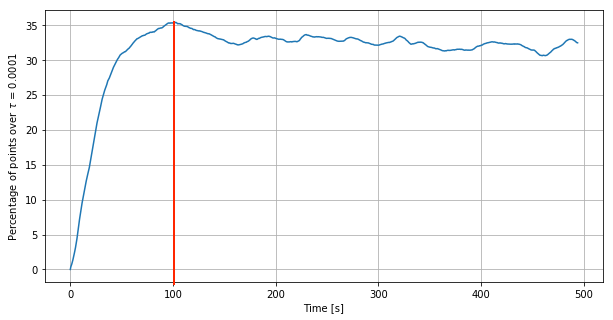
\includegraphics[width = 0.7 \textwidth]{figures/DataAnalysis/SumDataTime}
	\caption{Percentage of significant points in function of the time for $\tau = 10^{-4}$}
	\label{fig:sumtime}
\end{figure}


Furthermore, we decide to \textbf{round to zero} the values that are smaller than the previous threshold of $\tau = 10^{-4}$. This can be motivated by the fact that it will allow to use the sparsity of the data to make the algorithm faster. This means that we will approximatively set a 66\% of the tracer values to zero.\\

We try to find a trend in the data that we could exploit in the rest of the project. We plot for example the mean tracer value for each location in function to the distance to the origin of the tracer. This scatter plot can be seen on figure \ref{fig:tracerdistance}. 

\begin{figure}[]
\centering
	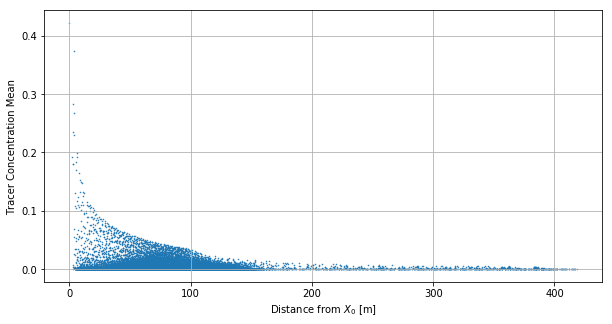
\includegraphics[width = 0.7 \textwidth]{figures/DataAnalysis/TracerMeanDistance}
	\caption{Mean value for each point in function of the distance to the tracer's origin}
	\label{fig:tracerdistance}
\end{figure}


As we can see there is no immediate trend that can be detected, so we proceed to a \textbf{centering of the Data} that will enable a faster processing of the covariance matrix. 















%%%%%%%%%%% CHAPTER : CONCLUSION
\chapter{Conclusion}

In this report, we have stated some of the research that was done in order to solve the sensor position optimisation problem. \\ 

The biggest challenge here is to make the algorithm scalable for optimising over $100'000$ sensor locations. It requires to develop strategies to make the GPs scalable. The main other challenge is to find a method to accurately estimate the covariance matrix. \\

I have implemented some of the optimisation algorithm proposed on a smaller dataset and with a poor estimation of the covariance function. It has given consistent results and has proven that once the main challenges, described earlier are solved, we will have a good optimisation algorithm for that kind of setups. 


%%%%%%%%%%%%%%%%%%%%%%%%%%%%%%%%%%%%
%\chapter{Further Developements}


%% bibliography
\bibliographystyle{apa}
\bibliography{bibliography}

\end{document}
